% textidote: ignore begin
\chapter{Problem statement}\label{ch:problem-statement}
% textidote: ignore end

To further narrow down and clarify the scope of the problem we are solving, reference is made to the problem delineation
and problem statement below.

% textidote: ignore begin
\section{Problem delineation}\label{sec:problem-delineation}
% textidote: ignore end

Chess can be taught and learned through various methods.
The biggest chess conglomerates have several learning features available for free for users of all levels.
However, they do not provide the multiplayer and learning experience simultaneously in any of their products.
Therefore, users who want to learn through multiplayer learning methods are not able to.

% textidote: ignore begin
\begin{figure}[htb]
    \centering
    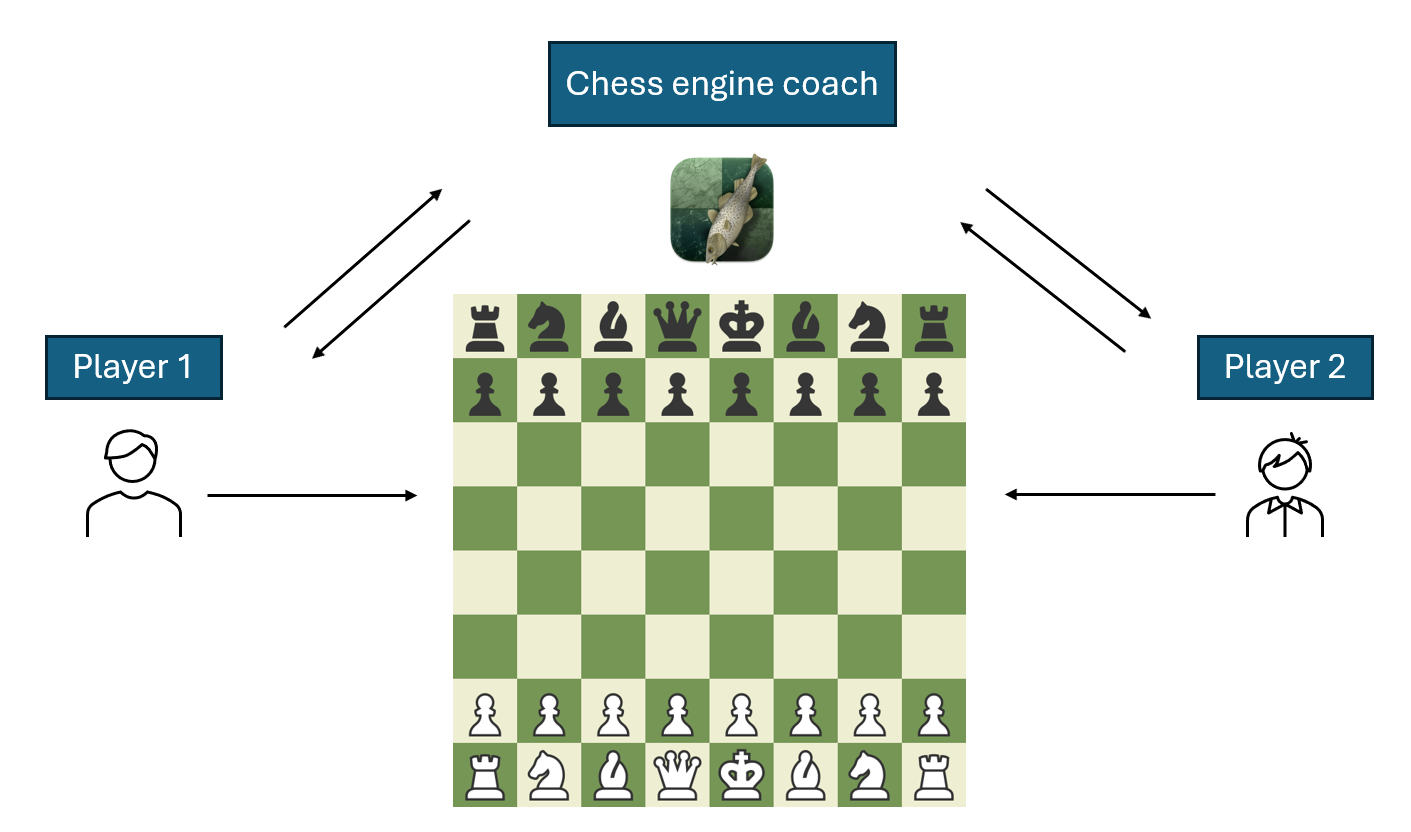
\includegraphics[width=0.75\textwidth]{solution-model}
    \caption{Visualising the solution.}\label{fig:visualising-the-solution}
\end{figure}
% textidote: ignore end

As seen in Figure~\ref{fig:visualising-the-solution} The goal if this project is to make it possible to have engine
assistance, while also being an online multiplayer game.

% textidote: ignore begin
\section{Problem statement}\label{sec:problem-statement}
% textidote: ignore end

How can we make an online multiplayer chess game for beginner players that facilitates learning chess using supervised
learning methods?
